\documentclass{article} % For LaTeX2e
\usepackage{iclr2020_conference,times}
\usepackage{graphicx}
\usepackage{placeins}
\usepackage{flafter}
\usepackage{pgf-pie}
\nocite{iemocap}
\nocite{binat}
\nocite{msp}
% Optional math commands from https://github.com/goodfeli/dlbook_notation.



\usepackage{hyperref}
\usepackage{url}

\title{Einfluss der Korpuszusammensetzung auf die Performance von audiobasierten Emotionserkennungssystemen}

% Authors must not appear in the submitted version. They should be hidden
% as long as the \iclrfinalcopy macro remains commented out below.
% Non-anonymous submissions will be rejected without review.

\author{Niels Lange \& Beate Zywietz\\
Institut für Maschinelle Sprachverarbeitung\\
Universität Stuttgart\\
Pfaffenwaldring 5, 70569 Stuttgart \\
\texttt{\{st158564, st155422\}@st.uni-stuttgart.de} \\
}
%The \author macro works with any number of authors. There are two commands
% used to separate the names and addresses of multiple authors: \And and \AND.
%
% Using \And between authors leaves it to \LaTeX{} to determine where to break
% the lines. Using \AND forces a linebreak at that point. So, if \LaTeX{}
% puts 3 of 4 authors names on the first line, and the last on the second
% line, try using \AND instead of \And before the third author name.

\newcommand{\fix}{\marginpar{FIX}}
\newcommand{\new}{\marginpar{NEW}}

\iclrfinalcopy % Uncomment for camera-ready version, but NOT for submission.
\begin{document}


\maketitle
\begin{abstract}
Im Rahmen dieses Projekts setzen wir uns mit dem Einfluss des Korpusaufbaus auf die Performance von Machine-Learning-basierten Emotionserkennungssystemen auseinander, indem wir mit verschiedenen Kombinationen von Classifiern und Korpora arbeiten. 

Wir verwenden die Datensätze IEMOCAP und MSP-IMPROV in Kombination mit zwei verschiedenen Machine-Learning-Verfahren, einem Decision Tree und einem Support Vector Classifier. Wir testen die Korpora sowohl einzeln als auch in Kombination miteinander sowie mit ausgeglichener Klassengröße. Zusätzlich untersuchen wir die Performance der Classifier auf Paaren von je zwei Emotionsklassen eines Korpus. Wir dokumentieren dabei, welche strukturellen Eigenschaften der verwendeten Korpora die Performance der Classifier beeinflussen und welche Emotionen korpusanabhängig besonders leicht oder schwer für die Classifier erkennbar zu sein scheinen. Abschließend stellen wir Vermutungen darüber an, auf welche Eigenschaften der Emotionen dies zurückzuführen sein könnte. 
\end{abstract}

\section{Einleitung und verwandte Literatur}
Emotionserkennung ist ein komplexe, anspruchsvolle Aufgabe. Auch uns Menschen gelingt es oft nicht, Gehörtes einstimmig einer Emotion zuzuordnen. 

Wie wir Stimuli interpretieren, ist hochgradig von unserem Wissen über den Gesprächskontext, unserem Verhältnis zu unserem Gesprächspartner und uns selbst als Person abhängig. Auch der kulturelle Hintergrund kann eine Rolle spielen. So wird zum Beispiel Russisch von Menschen, die selbst nicht Russisch sprechen, oft als aggressiv und übellaunig klingend beschrieben. 

Zudem gehen Emotionen in der Praxis fließend ineinander über. An welchem Punkt geht traurig in frustriert über? Wo frustriert in wütend? 

Machine Learning Classifier sind oft noch sehr unzuverlässig, wenn es darum geht, gesprochener Sprache eine Emotion zuzuordnen. 

In "Emotion recognition using a hierarchical binary decision tree approach"\citep{binat} arbeiten die Autoren mit hierarchischen binären Decision Trees auf dem Korpus \emph{IEMOCAP}, wobei die Emotionsklasse \emph{Neutral} am besten vom System erkannt wurde. \emph{Angry} und \emph{Happy} wurden oft miteinander verwechselt, ebenso \emph{Sad} und \emph{Neutral}. Insbesondere Happy wurde nur schlecht erkannt. 

Nachdem wir bei unseren ersten Versuchen mit Emotionserkennungssystemen nur sehr schlechte Ergebnisse erzielten, beschlossen wir, für unser Projekt den Einfluss verschiedener Eigenschaften des verwendeten Korpus auf die Performance von Classifiern näher zu untersuchen. 

Im Rahmen dieses Projekts verwenden wir zwei Machine-Learning-Verfahren, einen \emph{Decision Tree Classifier} und einen \emph{Support Vector Classifier}, und zwei Korpora von Sprachproben, IEMOCAP\citep{iemocap} und MSP-IMPROV\citep{msp}. Wir arbeiten sowohl mit Teilen der Korpora als auch mit Kombinationen, trainieren die Classifier auf die neuen Datensätze und vergleichen die Ergebnisse. So können wir herausfinden, welche strukturellen und qualitativen Eigenschaften der verwendeten Trainingskorpora und Testdaten Faktoren bei der Performance von Emotionserkennungssystemen sein können. 
\section{Methoden}
IEMOCAP ("interactive emotional dyadic motion capture
database") ist ein manuell annotierter englischsprachiger Korpus, der aus Sprachproben und der dazugehörigen mit einem Motion-Capture-Verfahren parallel aufgezeichneten Gestik und Mimik der Schauspieler besteht. Er enthält insgesamt circa 12 Stunden Material. Für dieses Projekt verwenden wir nur die Audiodateien dieses Korpus. 

Zehn Schauspieler, fünf Frauen und fünf Männer, wurden jeweils in Zweiergruppen aufgenommen, wie sie sowohl kurze Drehbücher vorspielten als auch Dialoge in vorgegebenen Szenarien improvisierten. 

Der Korpus ist in die Klassen \emph{Happiness}, \emph{Anger} (1103), \emph{Sadness} (1084), \emph{Neutral} (1708), \emph{Frustrated}, \emph{Disgust}, \emph{Fear}, \emph{Excitement} und \emph{Surprise} unterteilt. Für dieses Projekt werden Frustrated, Disgust, Fear und Surprise nicht verwendet. Excitement und Happiness werden von uns zu einer Klasse zusammengezogen (insgesamt 1636), da eine so kleinschrittige Unterteilung der Emotionen unserer Auffassung nach in diesem Fall nicht sinnvoll ist und der Vergleich mit MSP-IMPROV, unserem zweiten Korpus, sich so vereinfachen lässt. Insgesamt werden für dieses Projekt 5531 Sprachproben aus IEMOCAP verwendet. 
Im Hinblick auf die Audioqualität fällt auf, dass oft fetzenweise die Stimme des Gesprächspartners zu hören ist. Zudem ist teilweise Hintergrundrauschen hörbar, beispielsweise bei dem Material in Sad. \\ \\
Bei MSP-IMPROV handelt es sich ebenfalls um einen manuell annotierten englischsprachigen Korpus, der aus improvisierten Dialogen zwischen je zwei Schauspielern besteht. 

Die insgesamt zwölf Schauspieler (sechs Frauen und sechs Männer) wurden sowohl mit Mikrophon aufgenommen als auch gefilmt, wobei für dieses Projekt auch hier nur mit dem Audioteil gearbeitet wird. Die Schauspieler sollten sich in unterschiedliche Situationen hineinversetzen und Dialoge improvisieren, in die sie jedoch generische Sätze (z. B. "How can I not?"), die \emph{target sentences}, einbauen sollten, jedes Mal mit einer anderen Emotion. Die Autoren des Korpus erhofften sich so eine natürlichere Darstellung. 

Bei der Auswahl der target sentences wurden mehrere Kriterien beachtet: die Sätze sollten möglichst phonetisch divers sein und dabei generisch genug, um glaubwürdig in unterschiedlichen emotionalen Kontexten auftauchen zu können. 

Die Datenbank enthält außer den target sentences auch die improvisierten Teile der Szenarios, Aufnahmen, in denen die Schauspieler die target sentences vorlesen und Aufnahmen von natürlicher Sprache während der Pausen zwischen den Sessions. Letzterer Teil wird aufgrund von mangelhafter Audioqualität in diesem Projekt nicht verwendet. 

MSP-IMPROV unterscheidet vier Emotionsklassen: \emph{Happy}(1272), \emph{Sad}(819), \emph{Angry}(754) und \emph{Neutral}(2313). Insgesamt enthält der für dieses Projekt verwendete Teil von MSP-IMPROV 5158 Sprachproben. 

Auffällig bei der Audioqualität ist auch hier ein hörbares Hintergrundrauschen. Außerdem wechselt die Lautstärke zwischen den einzelnen Sprachproben stark. Zudem enthalten die Aufnahmen oft mehrere Sekunden Stille am Anfang oder Ende, da die Autoren auch die Mimik der Schauspieler filmten, während diese gerade nicht sprachen. Auch war im Hintergrund oft leise die Stimme des Gesprächspartners zu hören. \\ \\
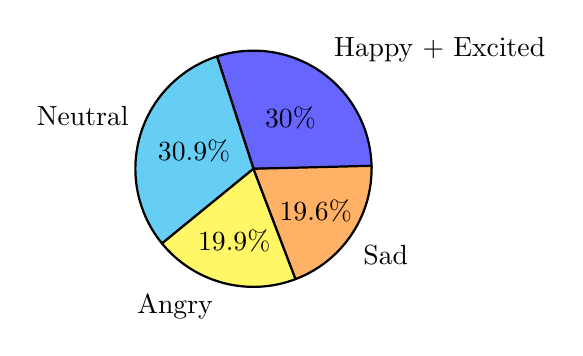
\begin{tikzpicture}
\pie [radius = 1.5]
    {30/Happy + Excited, 30.9/Neutral, 19.9/Angry, 19.6/Sad}
\end{tikzpicture}
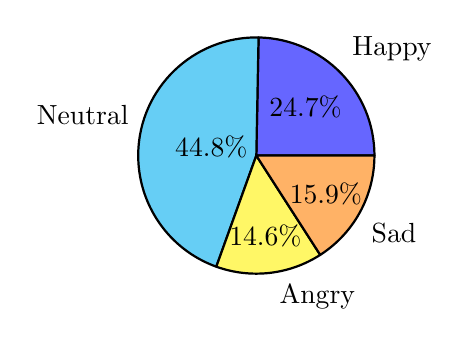
\begin{tikzpicture}
\pie [radius = 1.5]
    {24.7/Happy, 44.8/Neutral, 14.6/Angry, 15.9/Sad}
\end{tikzpicture} \\
Abb. 1: Prozentuale Verteilung der Emotionsklassen in IEMOCAP (links) und MSP-IMPROV (rechts). \\ \\
%1272/Happy, 2313/Neutral, 754/Angry, 819/Sad = 5158
%Angry 1103, Happy+Excited 1636, Neutr 1708, Sad 1084 = 5531
Beim Vergleich der beiden Korpora fällt auf, dass Emotionen teils unterschiedlich dargestellt wurden - während wir in IEMOCAP die "traurigen" Sprachproben als eher leise und in betroffenem Tonfall vorgetragen wahrnahmen, wirkten die Proben der gleichen Klasse in MSP-IMPROV eher aufgelöst und verzweifelt. \\ \\
Die beiden Datensätze werden mit zwei unterschiedlichen Machine-Learning-Verfahren benutzt, einem Decision Tree (DT) und einem Support Vector Classifier (SVC). Hierfür werden die in der Open Source Bibliothek Scikit-learn zur Verfügung gestellten Module Decision Tree Classifier (criterion = gini, min\_ samples\_ split = 100, max\_ depth = 50) und SVC (gamma = scale, C=275.0) verwendet. Die Module werden jeweils von Hand in Python 3 implementiert.  
Zur Extraktion der phonetischen Merkmale aus dem Korpus verwenden wir OpenSMILE. Wir benutzen jeweils 70\% der Korpora als Trainingsdaten und 30\% als Testdaten. 
\section{Versuche}
\subsection{IEMOCAP im Vergleich zu MSP-IMPROV}
\begin{tabular}{|r|llll|}
\hline
GS / DT & A & H & N & S \\
\hline
A & 194 & 69 & 53 & 11 \\
H & 88 & 219 & 156 & 39 \\
N & 34 & 134 & 307 & 62 \\
S & 11 & 21 & 97 & 165 \\
\hline
\end{tabular}
\begin{tabular}{|r|llll|}
\hline
GS / DT & A & H & N & S \\
\hline
A & 55 & 78 & 82 & 5 \\
H & 31 & 153 & 161 & 13 \\
N & 52 & 105 & 499 & 62 \\
S & 12 & 26 & 136 & 78 \\
\hline
\end{tabular} \\
Abb. 2: Konfusionsmatrix zu IEMOCAP (links) und MSP-IMPROV (rechts) mit Decision Tree, Reihen: Gold Standard, Zeilen: DT. \\ \\
Auffällig sind hier die stark unterschiedlichen Ergebnisse des Decision Trees im Bezug auf die Klassen Angry und Sad: Auf IEMOCAP erreicht Angry mit 0.6 den höchsten F1-Score und Sad den zweithöchsten mit 0.58, auf MSP-IMPROV wird Angry dagegen am schlechtesten erkannt (F1-Score von 0.3) und Sad am zweitschlechtesten (F1-Score 0.38). Für Happy und Neutral werden vergleichbare F1-Scores erreicht, 0.54 (IEMOCAP) und 0.42 (MSP-IMPROV) für Happy und 0.54 (IEMOCAP) und 0.63 (der höchste F1-Score auf MSP-IMPROV) für Neutral. 

Der Decision Tree performt auf IEMOCAP im Bezug auf die unterschiedlichen Klassen also verhältnismäßig ausgeglichen, während auf MSP-IMPROV größere Unterschiede zwischen den F1-Scores vorliegen. Insgesamt performt der Decision Tree auf IEMOCAP besser. \\ \\ \\
\begin{tabular}{|r|llll|}
\hline
GS / SVC & A & H & N & S \\
\hline
A & 113 & 138 & 47 & 29 \\
H & 33 & 240 & 173 & 56 \\
N & 4 & 124 & 287 & 122 \\
S & 1 & 21 & 68 & 204 \\
\hline
\end{tabular} 
\begin{tabular}{|r|llll|}
\hline
GS / SVC & A & H & N & S \\
\hline
A & 26 & 50 & 144 & 0 \\
H & 13 & 87 & 258 & 0 \\
N & 12 & 47 & 659 & 0 \\
S & 6 & 15 & 230 & 1 \\
\hline
\end{tabular} \\
Abb. 3: Konfusionsmatrix zu IEMOCAP (links) und MSP-IMPROV (rechts) mit Support Vector Classifier, Reihen: Gold Standard, Zeilen: SVC. \\ \\
Der Support Vector Classifier performt auf IEMOCAP für Sad am besten (F1-Score 0.58), auf MSP-IMPROV dagegen am schlechtesten (F1-Score 0.01). Happy und Angry werden sowohl auf IEMOCAP als auch auf MSP-IMPROV nur schlecht erkannt: Auf IEMOCAP haben die beiden Klassen mit 0.47 den niedrigsten F1-Score, auf MSP-IMPROV sogar nur 0.31 für Happy und 0.19 für Angry. 
Neutral wird auf beiden Korpora verhältnismäßig gut erkannt (F1-Score von 0.52 für IEMOCAP, 0.66 für MSP), allerdings gibt es hier viele \emph{false positives}. Auch dieser Classifier performt auf IEMOCAP ausgeglichener über die einzelnen Klassen und insgesamt besser als auf MSP-IMPROV. 

An dieser Stelle sei angemerkt, dass besonders in MSP-IMPROV die Menge an Daten pro Klasse stark schwankt und für Neutral mit Abstand das meiste Material existiert. 
\subsection{Paarweiser Vergleich der Emotionsklassen für IEMOCAP und MSP-IMPROV}
Um die Unterschiede in der Performance unserer Systeme auf den Korpora näher zu untersuchen führen wir Tests auf Emotionspaaren aus. Dabei nutzen wir jeweils nur die Daten aus zwei Emotionsklassen eines Datensatzes als Input, um genau zu erkennen, welche Emotionen besonders gut oder schlecht zu unterscheiden sind. 

Zunächst führen wir die Experimente mit dem Decision Tree durch.
Dabei lässt sich erkennen, dass das Emotionspaar aus den Klassen Happy und Angry mit beiden Datensätzen schwer zu unterscheiden ist (Recall 0.67 für Angry, 0.68 für Happy). Bei Training mit Daten aus MSP-IMPROV werden Daten aus Angry besonders oft als Happy vorhergesagt, Angry erreicht nur einen Recall von 0.48. 
Das Emotionspaar aus Angry und Sad wird hingegen mit beiden Datensätzen jeweils sehr gut unterschieden (Recall von 0.88 (Angry) und 0.87 (Sad) für IEMO, 0.71 (Angry) und 0.82 (Sad) für MSP-IMPROV). 
Wieder fällt auf, dass mit Training auf MSP-IMPROV viele Daten aus anderen Emotionsklassen oft fälschlicherweise Neutral zugeordnet werden. 

Wir wiederholen das Experiment mit dem SVC.
Wieder werden die Emotionen Happy und Angry auf beiden Datensätzen am schlechtesten unterschieden und Angry zu großen Teilen Happy zugeordnet (Recall von Angry 0.32, Recall von Happy 0.91, aber Precision 0.67). Auf MSP-IMPROV werden Daten aus Angry noch öfter als Happy vorhergesagt (Recall von Angry 0.15, Recall von Happy 0.96, Precision 0.66).
Vergleiche mit Neutral sind mit dem SVC auf MSP-IMPROV noch schlechter als mit dem DT. Daten aus Happy, Angry und Sad werden meistens als Neutral vorhergesagt, keine der drei Klassen erzielen einen Recall über 0.33.
Das Emotionspaar aus Neutral und Sad wird mit Training auf IEMOCAP gut unterschieden (Recall von Neutral 0.8, Recall von Sad 0.64), mit Training auf MSP-IMPROV hingegen wird die Klasse Sad überhaupt nicht benutzt und alle Daten werden Neutral zugewiesen. 

Auf beiden Systemen sind mit beiden Datensätzen die Klassen Happy und Angry besonders schwer zu unterscheiden. Angry und Sad hingegen werden in allen Versuchen gut unterschieden. Zudem können wir erneut erkennen, dass der Größenunterschied der Klassen die Performance unserer Systeme beeinflusst, besonders die des Support Vector Classifiers.
\subsection{Decision Tree und Support Vector Classifier auf MSP-IMPROV mit angeglichenen Klassengrößen}
\begin{tabular}{|r|llll|}
\hline
GS / DT & A & H & N & S \\
\hline
A & 134 & 55 & 15 & 21 \\
H & 61 & 120 & 25 & 15 \\
N & 23 & 43 & 130 & 52 \\
S & 37 & 40 & 32 & 102 \\
\hline
\end{tabular}
\begin{tabular}{|r|llll|}
\hline
GS / SVC & A & H & N & S \\
\hline
A & 120 & 56 & 19 & 30 \\
H & 47 & 102 & 29 & 43 \\
N & 10 & 30 & 138 & 70 \\
S & 34 & 31 & 52 & 94 \\
\hline
\end{tabular} \\
Abb. 4: Konfusionsmatrix von DT (links) und SVC (rechts) auf MSP-IMPROV mit angeglichener Klassengröße, Reihen: Gold Standard, Zeilen: DT. \\ \\
Um zu überprüfen welchen Einfluss die ungleiche Klassenverteilung in MSP-IMPROV auf unsere Ergebnisse hat, wiederholen wir unsere Experimente mit angeglichenen Klassengrößen. Dazu beschränken wir alle Klassen aus MSP auf die Größe der kleinsten Klasse, welche 754 Datenpunkte enthält. 

Zunächst testen wir beide Systeme auf den beschränkten Klassen. 

Wie in Abb. X (!!!ref einfügen!!!) zu sehen ist performt der DT nun auf allen Klassen deutlich besser, die Performance ist insgesamt ausgeglichener. Vor allem Sad und Angry werden deutlich besser erkannt.
Auf Neutral performt das System weiterhin am besten, am schlechtesten werden Sad und Happy erkannt. Mit der Begrenzung performt der DT auf MSP-IMPROV nun genauso gut wie auf IEMOCAP. 

Wie beim DT ist die Performance des SVC deutlich ausgeglichener. Alle Emotionen werden deutlich besser erkannt, wobei Neutral noch immer am besten und Sad am schlechtesten erkannt wird. 

Das Angleichen der Klassengrößen hat die Performance deutlich verbessert.
Beim DT hat sich auch das Verhältnis der Performance auf den Klassen geändert, sodass die Klasse Angry, die zuvor am schlechtesten performt hat, nun besser erkannt wird als Happy und Sad. Obwohl die Performance nun der auf IEMOCAP ähnelt, wird Sad von beiden Systemen, trainiert auf MSP-IMPROV, am schlechtesten erkannt. Dieser Unterschied scheint Korpusabhängig zu sein. 
\subsection{Emotionspaare mit angeglichenen Klassengrößen}
Nachdem die Begrenzung der Klassengrößen in MSP-IMPROV bei beiden Systemen zu einer deutlichen Verbesserung der Performance geführt hat, führen wir nun wie in (REF) Tests auf Emotionspaaren durch. 

Der Decision Tree unterscheidet das Emotionspaar aus den Klassen Happy und Angry weiterhin am schlechtesten. Emotionen im Emotionspaar mit Neutral werden nun deutlich besser erkannt, besonders Happy und Neutral werden besser unterschieden. 

Wie zuvor wird auch mit dem Support Vector Classifier das Emotionspaar aus Happy und Angry noch immer am schlechtesten unterschieden. Auch hier wird in Emotionspaaren, die Neutral enthalten, nun deutlich besser zwischen den beiden Emotionen unterschieden. Im Emotionspaar aus Sad und Neutral werden beide Klassen nun gleich gut erkannt. 

Auch für die Emotionspaare hat das Anpassen der Klassengrößen die gesamte Performance deutlich verbessert. Das Emotionspaar aus Happy und Angry wird wie in (REF) am schlechtesten unterschieden.
\subsection{Decision Tree und Support Vector Classifier auf Kombinationen der Korpora}
\begin{tabular}{|r|llll|}
\hline
GS / DT & A & H & N & S \\
\hline
A & 241 & 467 & 35 & 3 \\
H & 330 & 836 & 92 & 3 \\
N & 537 & 1429 & 307 & 20 \\
S & 112 & 534 & 137 & 24 \\
\hline
\end{tabular}
\begin{tabular}{|r|llll|}
\hline
GS / DT & A & H & N & S \\
\hline
A & 178 & 411 & 278 & 224 \\
H & 106 & 466 & 607 & 444 \\
N & 100 & 228 & 656 & 706 \\
S & 69 & 54 & 320 & 629 \\
\hline
\end{tabular} \\
\begin{tabular}{|r|llll|}
\hline
GS / DT & A & H & N & S \\
\hline
A & 254 & 133 & 138 & 25 \\
H & 180 & 317 & 312 & 76 \\
N & 104 & 214 & 722 & 161 \\
S & 22 & 56 & 250 & 243 \\
\hline
\end{tabular} \\
Abb. 5: Konfusionsmatrix zu DT, links trainiert auf IEMOCAP und getestet auf MSP-IMPROV, rechts trainiert auf MSP-IMPROV und getestet auf IEMOCAP, unten trainiert und getestet auf Kombination beider Korpora, Reihen: Gold Standard, Zeilen: SVC. \\ \\
Der auf IEMOCAP trainierte Decision Tree performt auf MSP-IMPROV (unbegrenzt) am besten für Happy (Höchster F1-Score mit 0.37, höchster Recall mit 0.66, allerdings niedrige Precision mit 0.26). Angry erreicht einen Recall von 0.32 und mit 0.2 die schlechteste Precision. Neutral und Sad erreichen mit 0.13 und 0.03 die schlechtesten Werte für Recall und mit 0.21 und 0.06 die schlechtesten Werte für den F1-Score, erzielen aber mit 0.54 und 0.48 die höchste Precision. 
Insgesamt werden die Daten anderer Klassen nun meist als Happy klassifiziert. Daten aus Happy werden oft unter Angry eingeordnet. 

Trainiert man den DT auf MSP-IMPROV und testet ihn dann auf IEMOCAP, erreicht Sad mit 0.59 den höchsten Recall und trotz der niedrigsten Precision (0.31) mit 0.41 den höchsten F1-Score. 
Happy und Angry erreichen hier mit 0.4 und 0.39 die höchste Precision, aber mit 0.29 und 0.16 den niedrigsten Recall. F1-Scores sind 0.34 für Happy und 0.23 für Angry. Neutral wird mit Precision 0.35, Recall 0.39 und F1-Score 0.37 verhältnismäßig gut erkannt. 
Der DT verwechselt oft Sad und Neutral miteinander. Angry wird vor allem Happy zugeordnet. Happy wird hauptsächlich als Neutral erkannt. 

Trainiert und testet man den DT auf einer Kombination beider Korpora, wird Neutral mit einem F1-Score von 0.55, einem Recall von 0.6 und einer Precision von 0.51 am besten erkannt. Happy wird am schlechtesten erkannt (Precision 0.44, Recall 0.36, F1-Score 0.4) und oft Neutral zugeordnet. Sad (Precision 0.48, Recall 0.43, F1-Score 0.45) und Angry (Precision 0.45, Recall 0.46, F1-Score 0.46) werden verhältnismäßig gut erkannt, wobei Sad häufiger Neutral zugeordnet wird als sich selbst und Angry häufig Neutral und Happy. \\ \\ \\
\begin{tabular}{|r|llll|}
\hline
GS / SVC & A & H & N & S \\
\hline
A & 495 & 203 & 42 & 6 \\
H & 684 & 419 & 156 & 2 \\
N & 787 & 783 & 700 & 23 \\
S & 186 & 402 & 206 & 13 \\
\hline
\end{tabular}
\begin{tabular}{|r|llll|}
\hline
GS / SVC & A & H & N & S \\
\hline
A & 1 & 313 & 777 & 0 \\
H & 2 & 243 & 1376 & 2 \\
N & 2 & 69 & 1618 & 1 \\
S & 0 & 49 & 1021 & 2 \\
\hline
\end{tabular} \\
\begin{tabular}{|r|llll|}
\hline
GS / SVC & A & H & N & S \\
\hline
A & 99 & 226 & 211 & 14 \\
H & 65 & 321 & 460 & 39 \\
N & 23 & 179 & 918 & 81 \\
S & 8 & 40 & 383 & 140 \\
\hline
\end{tabular} \\
Abb. 6: Konfusionsmatrix zu SVC, links trainiert auf IEMOCAP und getestet auf MSP-IMPROV, rechts trainiert auf MSP-IMPROV und getestet auf IEMOCAP, unten trainiert und getestet auf Kombination beider Korpora, Reihen: Gold Standard, Zeilen: SVC. \\ \\

Testet man den auf IEMOCAP trainierten SVC auf MSP-IMPROV, wird Sad sehr schlecht erkannt (Recall 0.02)und hauptsächlich Happy zugeordnet. Neutral wird ca. zu je einem Drittel Angry, Happy und sich selbst zugeordnet (Recall 0.31). Happy (Recall 0.33) wird häufiger Angry zugeordnet als sich selbst. Angry wird gut erkannt (Recall 0.66) und teils Happy zugeordnet. 

Testet man den auf MSP-IMPROV trainierten SVC auf IEMOCAP, werden Angry und Sad fast gar nicht verwendet (Precision je 0.2 und 0.4, Recall und F1-Score jedoch für beide 0). Happy wird fast vollständig Neutral zugeordnet (Recall von 0.15). Neutral wird mit einem Recall von 0.96 sehr gut erkannt (F1-Score 0.5). 

Trainiert und testet man den SVC auf beiden Korpora, wird Neutral mit einem Recall von 0.76 (F1-Score 0.58) am besten erkannt. Angry wird mit einem Recall von 0.18 (F1-Score 0.27) am schlechtesten erkannt und meist Happy oder Neutral zugeordnet. Sad wird ebenfalls nur schlecht erkannt (Recall 0.25, F1-Score 0.33) und meist Neutral zugeordnet. Happy wird häufiger richtig eingeordnet (Recall 0.36, F1-Score 0.39), aber ebenfalls meist Neutral zugeordnet. 
\section{Diskussion}
Durch unsere Experimente können wir feststellen, dass sich Unterschiede in den Klassengrößen stark auf die Performance unserer Systeme auswirken können. Werden diese Unterschiede ausgeglichen, performen beide Systeme besser und über die verschiedenen Emotionsklassen ausgeglichener. Zudem können wir einige korpusabhängige Unterschiede in unseren Ergebnissen finden. Werden die Systeme auf IEMOCAP trainiert, wird Sad sehr gut erkannt (F1-Score 0.58), beim Training auf MSP-IMPROV wird Sad auch mit angeglichenen Klassengrößen eher schlecht erkannt (F1-Score 0.42). Im Vergleich der einzelnen Emotionspaare wird das Paar aus Happy und Neutral von beiden Systemen mit Training auf MSP-IMPROV sehr gut unterschieden (Accuracy 0.79), während das Paar unter Nutzung der Daten aus IEMOCAP verhältnismäßig schlecht unterschieden wird (Accuracy 0.67). 

Bei der Kombination beider Datensätze lassen sich weitere korpusabhängige Unterschiede finden. Hier fällt auf, dass mit Training auf MSP-IMPROV und Testen mit IEMOCAP Sad sehr oft Neutral zugeordnet wird. Die Emotion Sad wird in MSP-IMPROV und IEMOCAP recht unterschiedlich dargestellt: In IEMOCAP sind die Aufnahmen aus der Klasse Sad eher leise und niedergeschlagen gespielt, in MSP-IMPROV hingegen wird Sad laut und verzweifelt dargestellt. Vermutlich werden deshalb die eher leisen Testdaten aus der Klasse Sad hier in die ebenfalls als ruhig dargestellte Klasse Neutral eingeordnet. 

In unseren Experimenten fallen ebenfalls mehrere Emotionen auf, die system- und korpusunabhängig immer besonders gut oder schlecht performen zu scheinen. So wird Happy sehr oft mit anderen Emotionen verwechselt. Das Emotionspaar Happy und Angry wird in sämtlichen Versuchen am schlechtesten auseinander gehalten. Dies könnte daran liegen, dass beide Emotionen eher "laut"/"energiegeladen" sind. Sad ist die "leiseste" Emotion und lässt sich demnach recht gut von Angry unterscheiden. 

Um diese Faktoren weiter untersuchen und sichere Aussagen treffen zu können, wäre es sinnvoll mit weiteren Korpora und Machine-Learning-Verfahren zu experimentieren und die Ergebnisse zu vergleichen. Eine bessere Aufbereitung der verwendeten Datensätze beugt der Fehlerquelle durch schlechte Audioqualität vor, die uns vor allem in MSP-IMPROV aufgefallen ist. Da wir keine genauen Analysen der Merkmale unserer Daten durchgeführt haben, basieren unsere Theorien auf subjektiver Wahrnehmung und sollten durch weitere Experimente mit Fokus auf bestimmte Eigenschaften der Emotionen überprüft werden.
\section{Zusammenfassung}
Wir haben unter Zuhilfenahme eines Decision Trees und eines Support Vector Classifiers untersucht, welchen Einfluss die Struktur der von uns verwendeten Korpora auf die Performance der Classifier hat und welche Emotionen korpusunabhängig besonders einfach oder schwierig erkennbar zu sein scheinen. 

Dabei haben wir festgestellt, dass die Mengenverteilung der Daten über die verschiedenen Emotionsklassen eine große Rolle spielt. In unserem Fall enthielt die Klasse Neutral aus MSP-IMPROV zum Beispiel deutlich mehr Material als die anderen Klassen des Korpus, was unsere Resultate stark beeinflusste. 

In einem weiteren Experiment haben wir die Klassengrößen an die der Klasse mit den wenigsten Daten angeglichen, sodass alle Klassen gleich viele Datenpunkte enthielten. Dadurch konnten wir konkretere Hinweise auf korpusabhängige und korpusunabhängige Faktoren in unseren Ergebnissen erhalten. Des weiteren haben wir die Korpora kombiniert und jeweils und unsere Classifier je auf dem einen trainiert und auf dem anderen getestet, um zusätzliche Erkenntnisse über die Unterschiede der Korpora zu erhalten. 

So stellten wir fest, dass die  als "laut"/"energiegeladen" gespielte Emotion Angry von den Classifiern verhältnismäßig gut von der "leise"/"niedergeschlagene" gespielten Emotion Sad unterschieden wird, aber dafür schwer von Happy, was ebenfalls als eher "laut"/"energiegeladen" gespielt wurde, zu unterscheiden ist. 

Uns fiel zudem auf, dass Sad in IEMOCAP und MSV-IMPROV unterschiedlich dargestellt wurde (leise und niedergeschlagen gegen laut und verzweifelt), was erklären kann, weshalb Sad beim Training auf MSP-IMPROV und Testen auf IEMOCAP nur sehr schlecht erkannt wurde. 

Wir halten fest, dass die Korpuszusammensetzung einen großen Einfluss auf die Performance von Emotionserkennungssystemen hat. 

Um den unbeabsichtigten Einfluss von Unterschieden zwischen verschiedenen Korpora auf die Performance zu minimieren und Experimente somit vergleichbarer zu machen sollte zum einen auf eine ausgeglichene Datenverteilung zwischen den Klassen geachtet werden, zum anderen müsste es einen Weg geben, Emotionen zu standardisieren. Da Emotionen jedoch von jeder Sprache, Kultur und sogar von jedem Mensch unterschiedlich ausgedrückt und wahrgenommen werden, wird es kaum möglich sein, Fehler dieser Art gänzlich zu vermeiden.
\pagebreak
\tableofcontents
\pagebreak
\bibliography{iclr2020_conference}
\bibliographystyle{iclr2020_conference}

\end{document}
